%% LaTeX-Beamer template for KIT design
%% by Erik Burger, Christian Hammer
%% title picture by Klaus Krogmann
%%
%% version 2.1
%%
%% mostly compatible to KIT corporate design v2.0
%% http://intranet.kit.edu/gestaltungsrichtlinien.php
%%
%% Problems, bugs and comments to
%% burger@kit.edu

\documentclass[18pt]{beamer}
\usepackage[utf8]{inputenc}

%% SLIDE FORMAT

% use 'beamerthemekit' for standard 4:3 ratio
% for widescreen slides (16:9), use 'beamerthemekitwide'

\usepackage{templates/beamerthemekit}
% \usepackage{templates/beamerthemekitwide}

\usepackage{graphicx}

%% TITLE PICTURE

% if a custom picture is to be used on the title page, copy it into the 'logos'
% directory, in the line below, replace 'mypicture' with the
% filename (without extension) and uncomment the following line
% (picture proportions: 63 : 20 for standard, 169 : 40 for wide
% *.eps format if you use latex+dvips+ps2pdf,
% *.jpg/*.png/*.pdf if you use pdflatex)

%\titleimage{mypicture}

%% TITLE LOGO

% for a custom logo on the front page, copy your file into the 'logos'
% directory, insert the filename in the line below and uncomment it

\titlelogo{GAns}

% (*.eps format if you use latex+dvips+ps2pdf,
% *.jpg/*.png/*.pdf if you use pdflatex)

%% TikZ INTEGRATION

% use these packages for PCM symbols and UML classes
% \usepackage{templates/tikzkit}
% \usepackage{templates/tikzuml}
\usepackage{tikz}

% the presentation starts here

\title[Graph von Ansicht]{Graph von Ansicht:\\ Visualisierung von Programmabhängigkeitsgraphen}
\subtitle{}
\author{Nicolas Boltz, Jonas Fehrenbach, Sven Kummetz, Jonas Meier, Lucas Steinmann}

\institute{}

% Bibliography

\bibliographystyle{plain}
\graphicspath{{resourcen/}}
%\usepackage[citestyle=authoryear,bibstyle=numeric,hyperref,backend=biber]{biblatex}
%\addbibresource{templates/example.bib}
%\bibhang1em

\begin{document}

% change the following line to "ngerman" for German style date and logos
\selectlanguage{ngerman}

%title page
\begin{frame}
\titlepage
\end{frame}

\author{Nicolas B., Jonas F., Sven K., Jonas M., Lucas S.}

\section{Einleitung/Zielbestimmung}
\begin{frame}{Ziele}
  \begin{itemize}
    \item Programmabhängigkeitsgraphen anschaulich und strukturiert darzustellen
    \pause
    \pause
    \pause
    \item Heuristische Strategien zur Optimierungen von
      \begin{itemize}
        \item Kantenkreuzungen
        \item Kantenlängen
        \item Durchsetzung des hierarchischen Layouts (z.B. wenige Aufwärtskanten)
      \end{itemize}
      mit dem Framework von Sugiyama.
    \pause
    \item Mustererkennung für Subgraphen
    \pause
    \item intuitive Navigation
  \end{itemize}
  \only<2> {
    \begin{tikzpicture}[remember picture,overlay]
      \node at (current page.center) {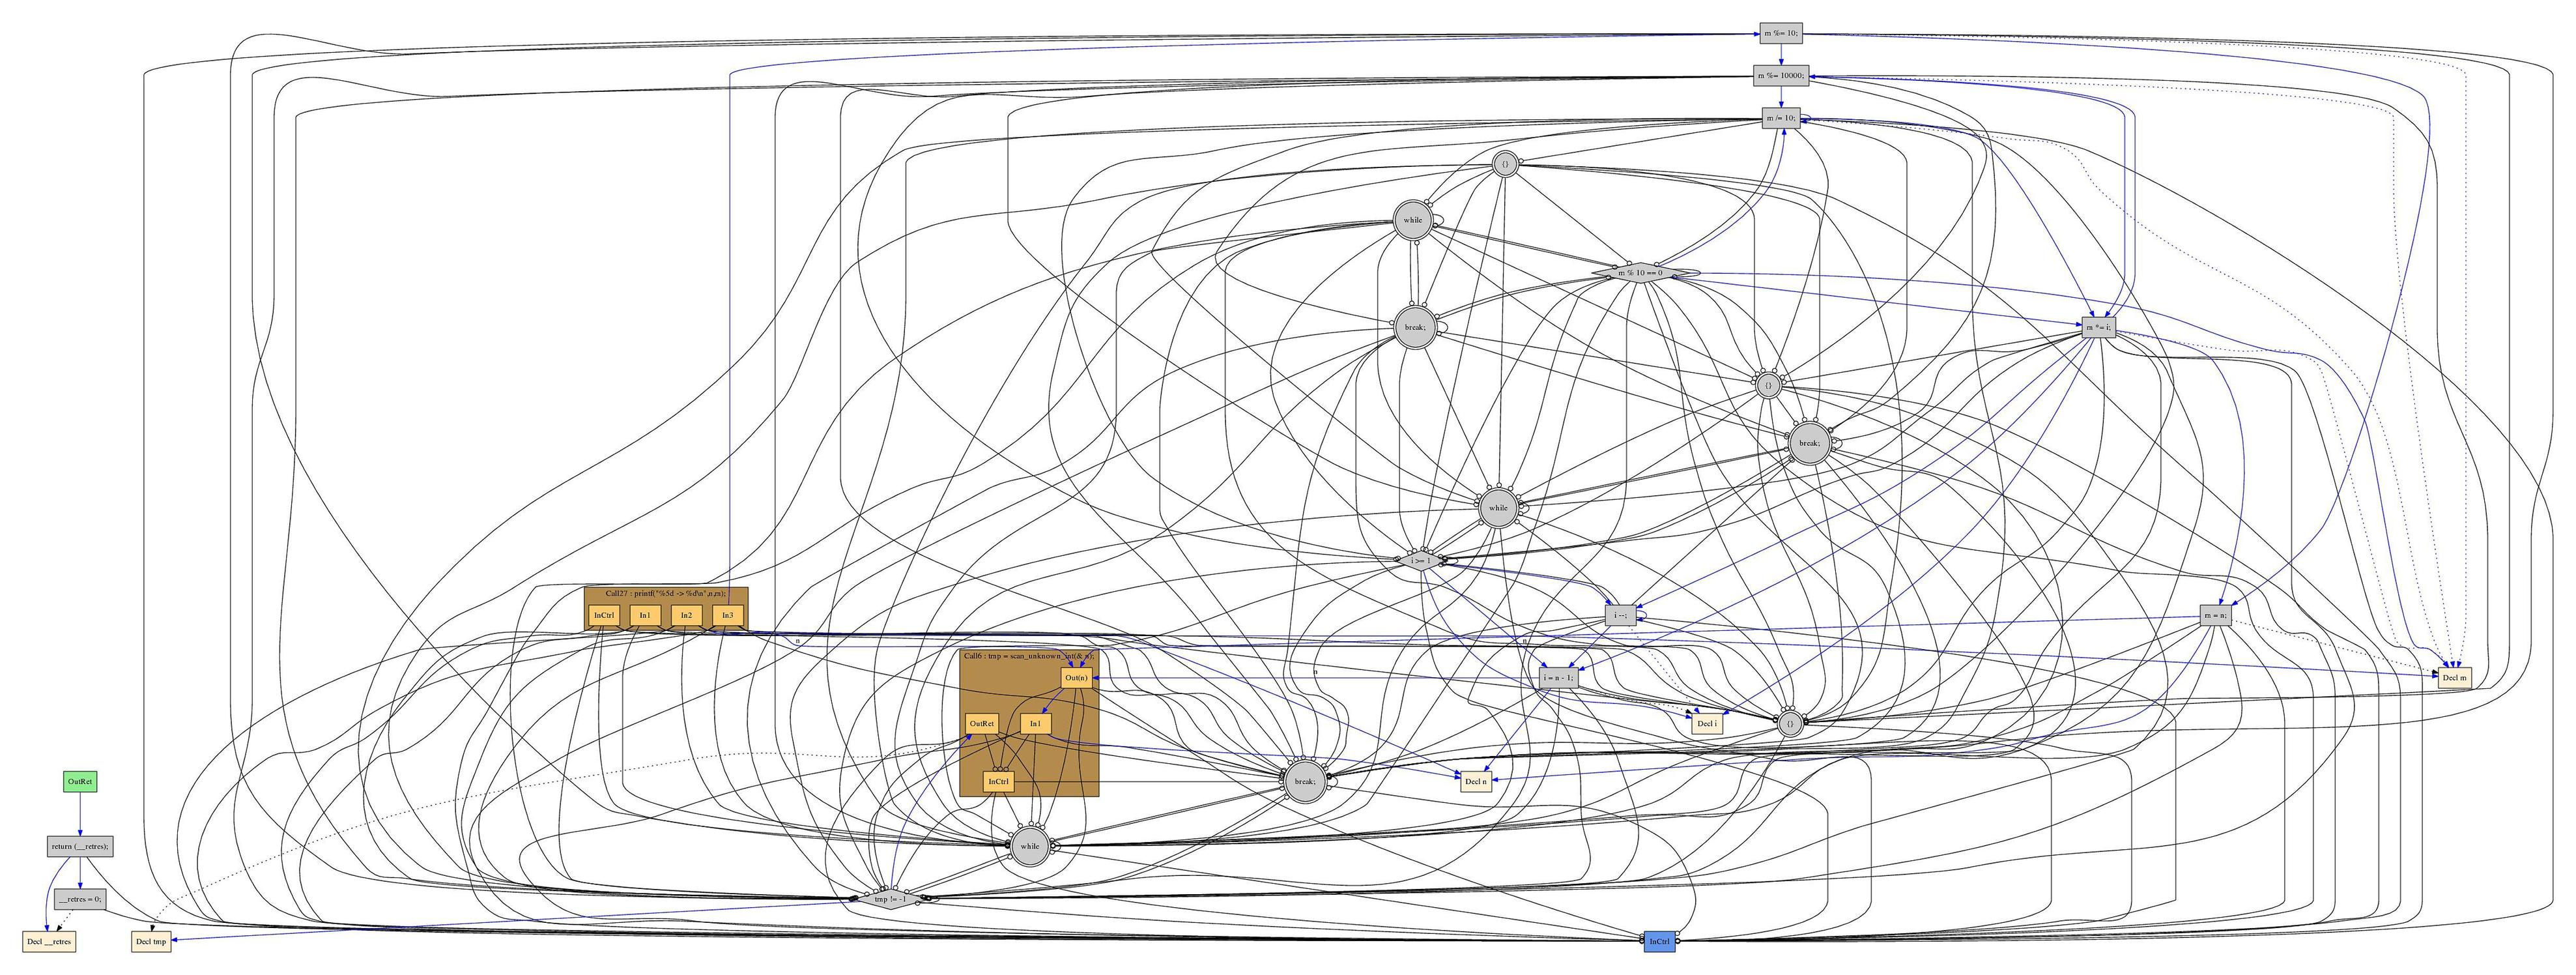
\includegraphics[width=330pt]{resourcen/gegenbeispiel_b.jpg}};
    \end{tikzpicture}
  }
\end{frame}

\section{Benutzerschnittstellen}
\begin{frame}{Benutzerschnittstellen}
  \begin{tabular}[t]{cc}

      \begin{minipage}[t]{0.45\textwidth}
      Kommandozeile \\
      \raisebox{-.5\height}{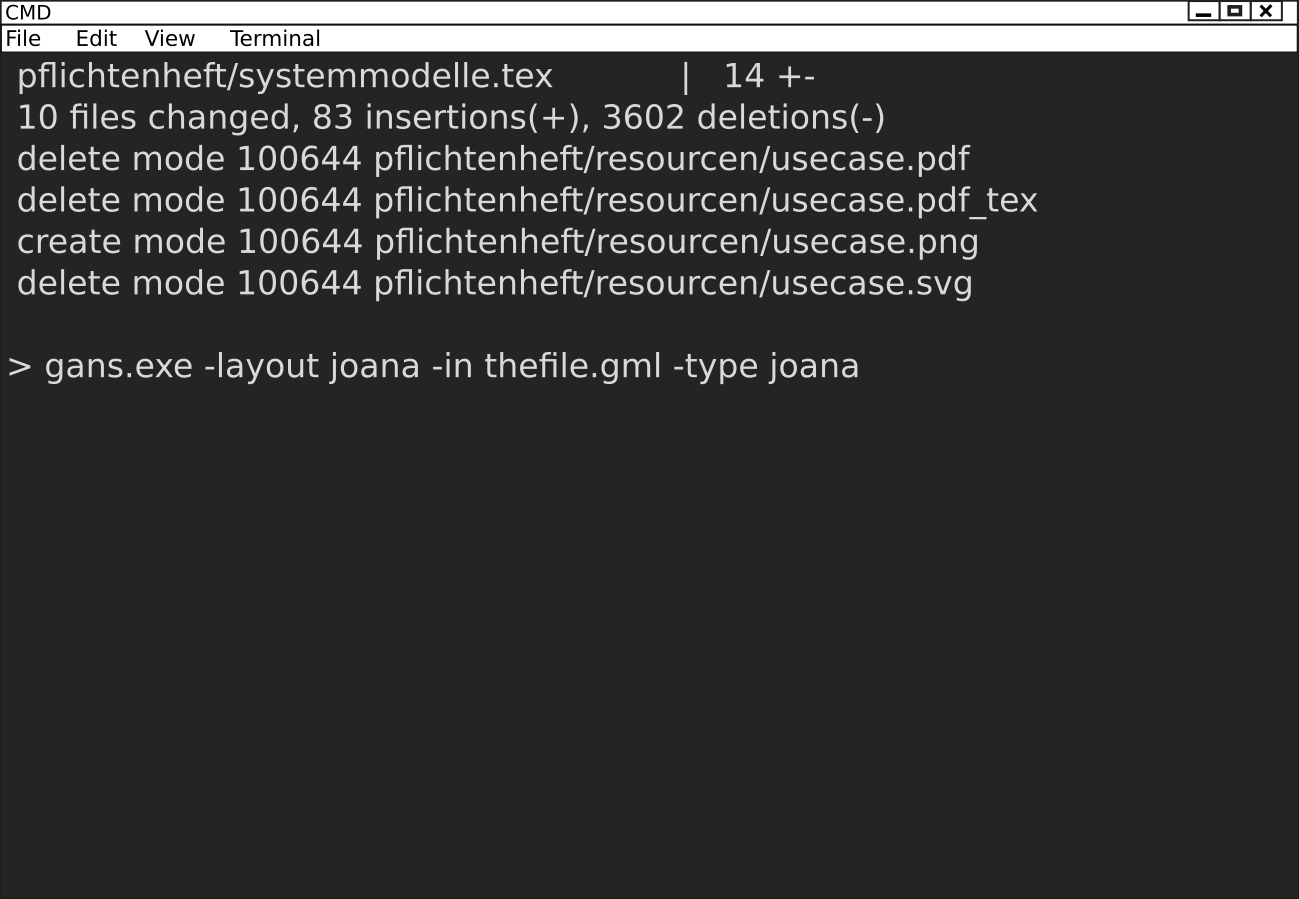
\includegraphics[width=150pt]{resourcen/cmd.png}}

      \begin{itemize}
        \item schnelle Möglichkeit Graphen zu layouten
        \item Massenverarbeitung von Dateien
      \end{itemize}
      \end{minipage}
    \pause
    &

    \begin{minipage}[t]{0.45\textwidth}
     \visible<2->{
       GUI \\
      \raisebox{-.5\height}{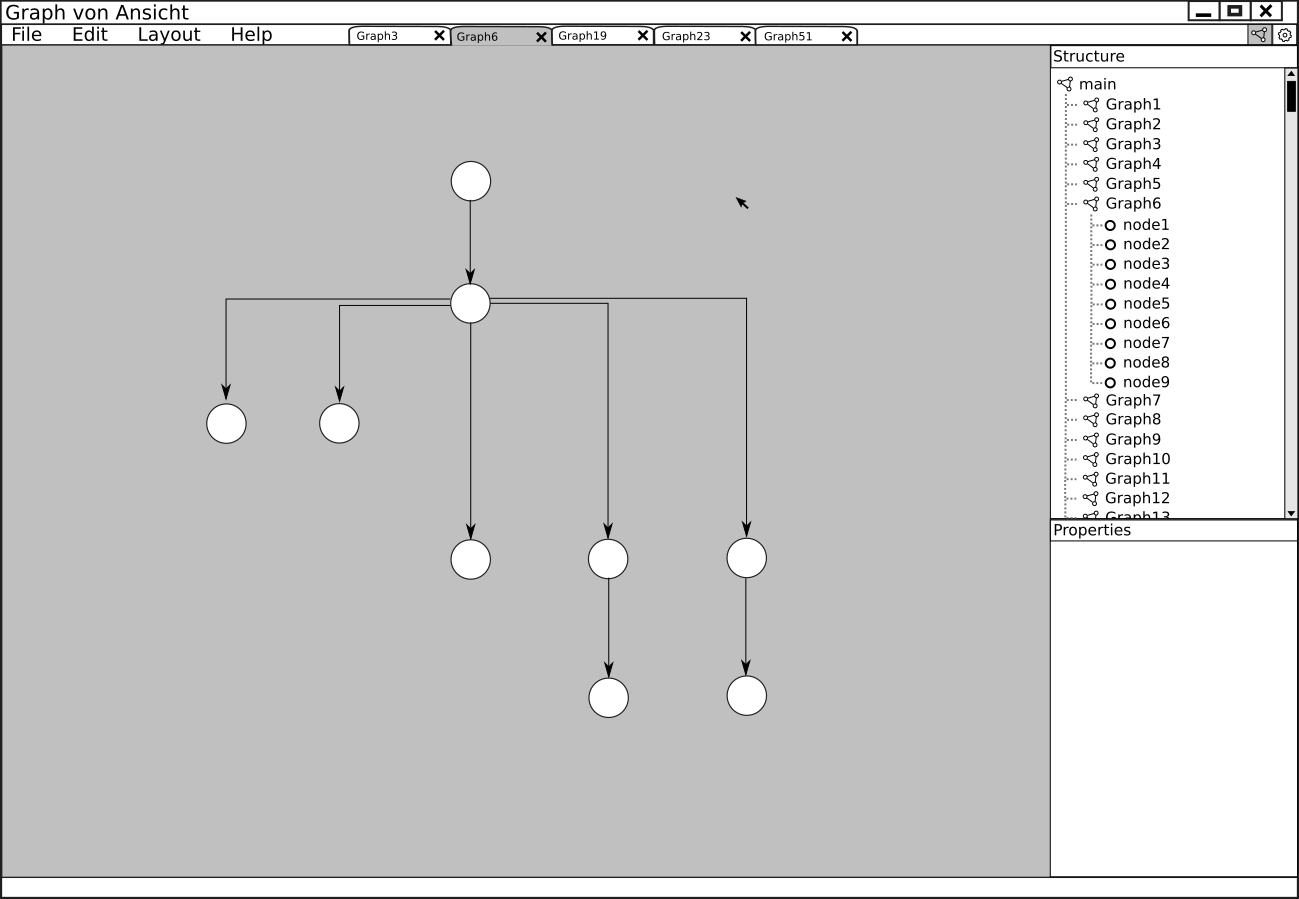
\includegraphics[width=150pt]{resourcen/gui.png}}

      \begin{itemize}
        \item Darstellung der Graphen
        \item interaktives Interface zur Anpassung des Layouts
      \end{itemize}
      }
      \end{minipage}
    \\
  \end{tabular}
\end{frame}

\begin{frame}{Komponenten}
  \only<1>{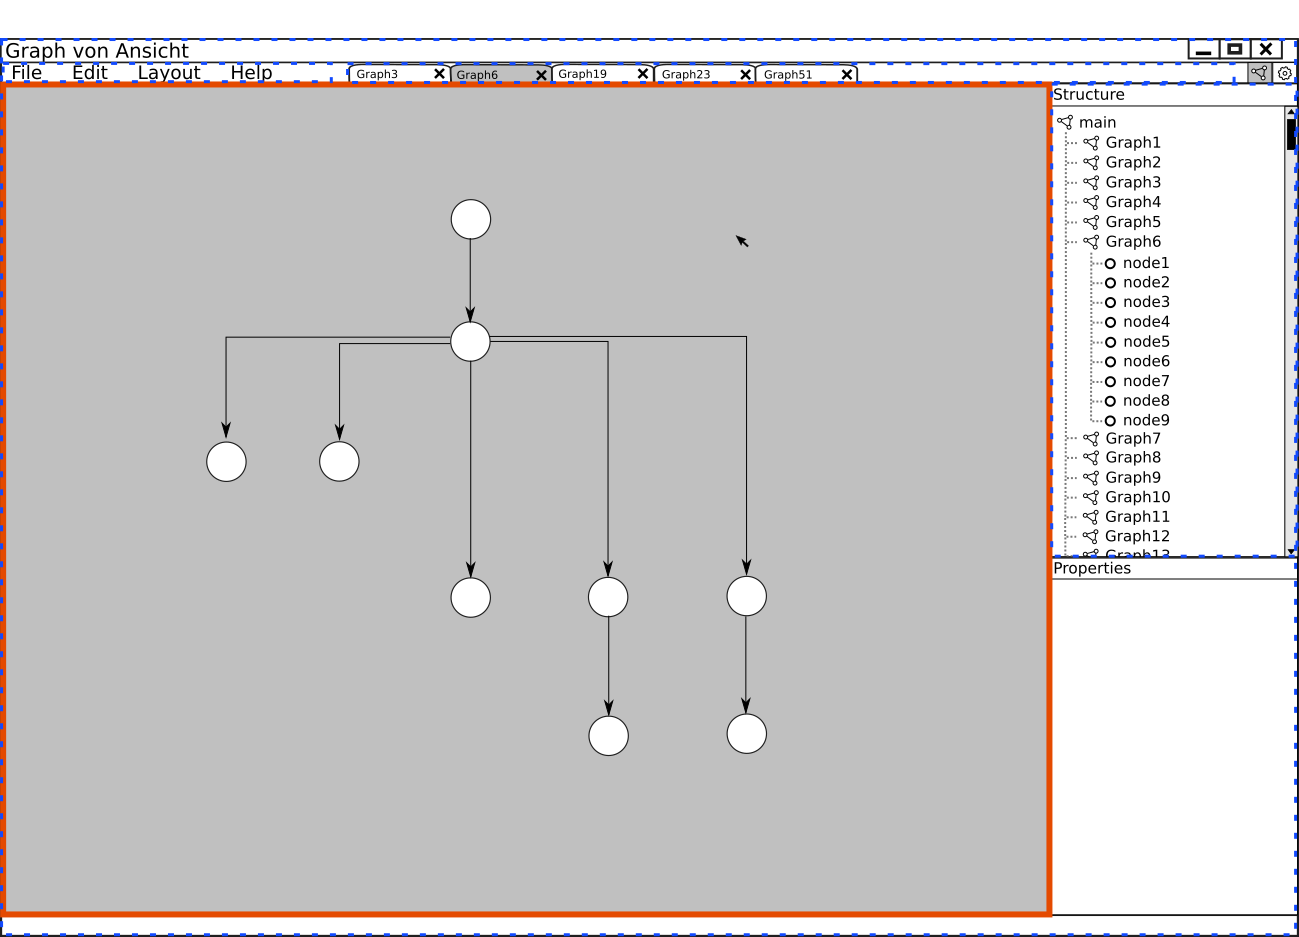
\includegraphics[width=280pt]{resourcen/gui_view_treeview_a.png}}
  \only<2>{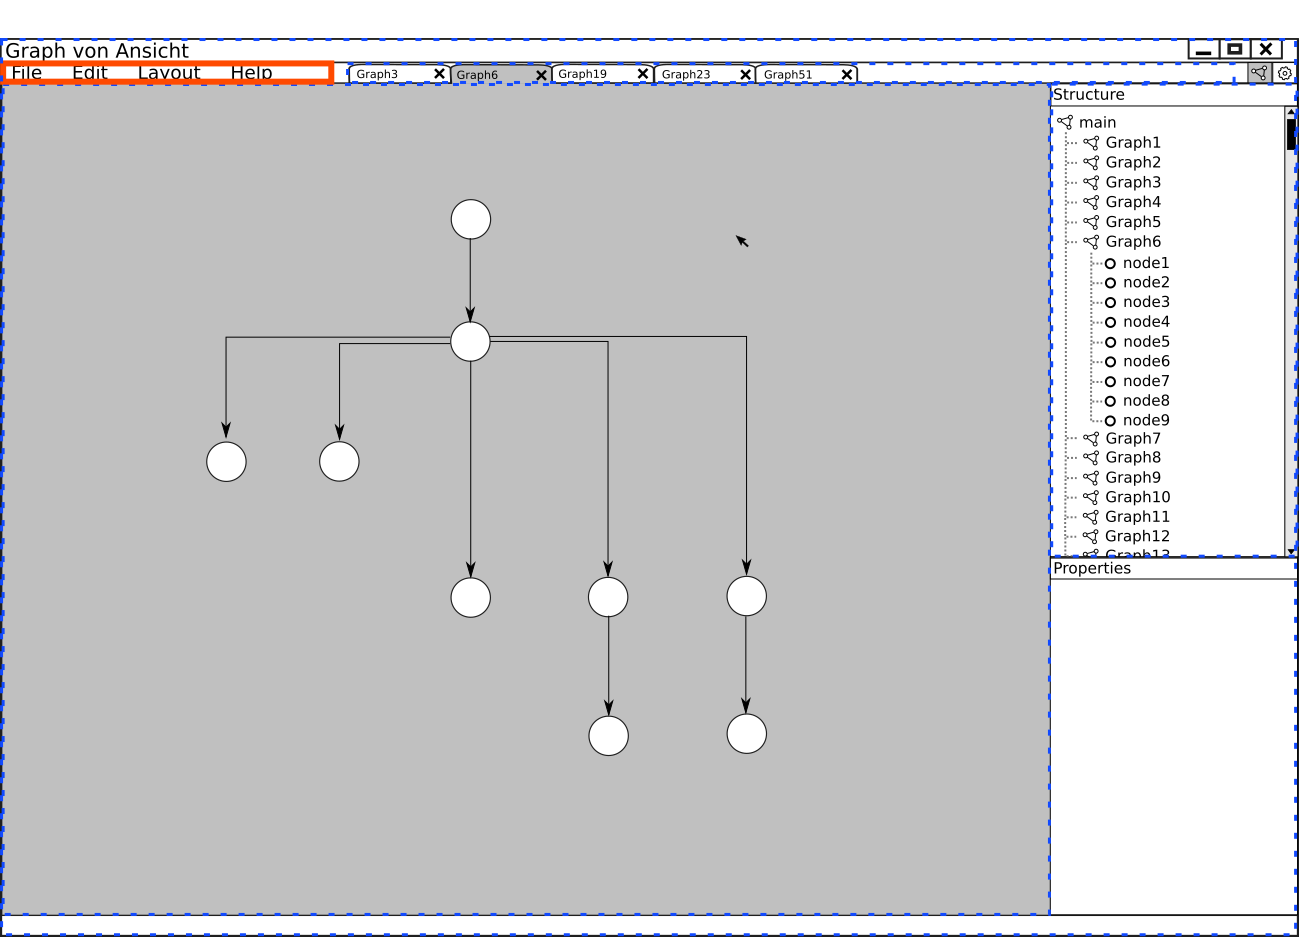
\includegraphics[width=280pt]{resourcen/gui_view_treeview_b.png}}
  \only<3>{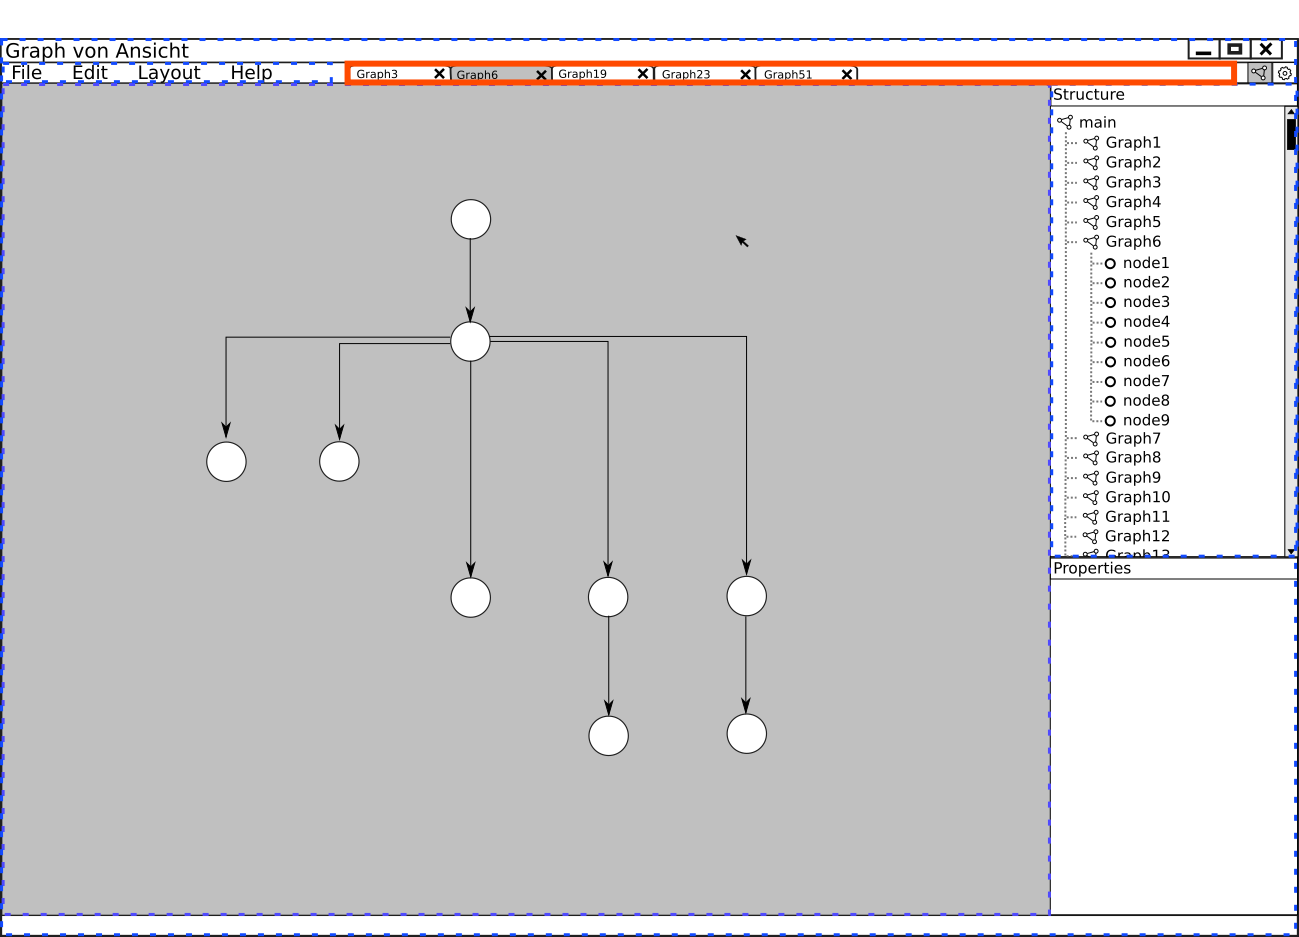
\includegraphics[width=280pt]{resourcen/gui_view_treeview_c.png}}
  \only<4>{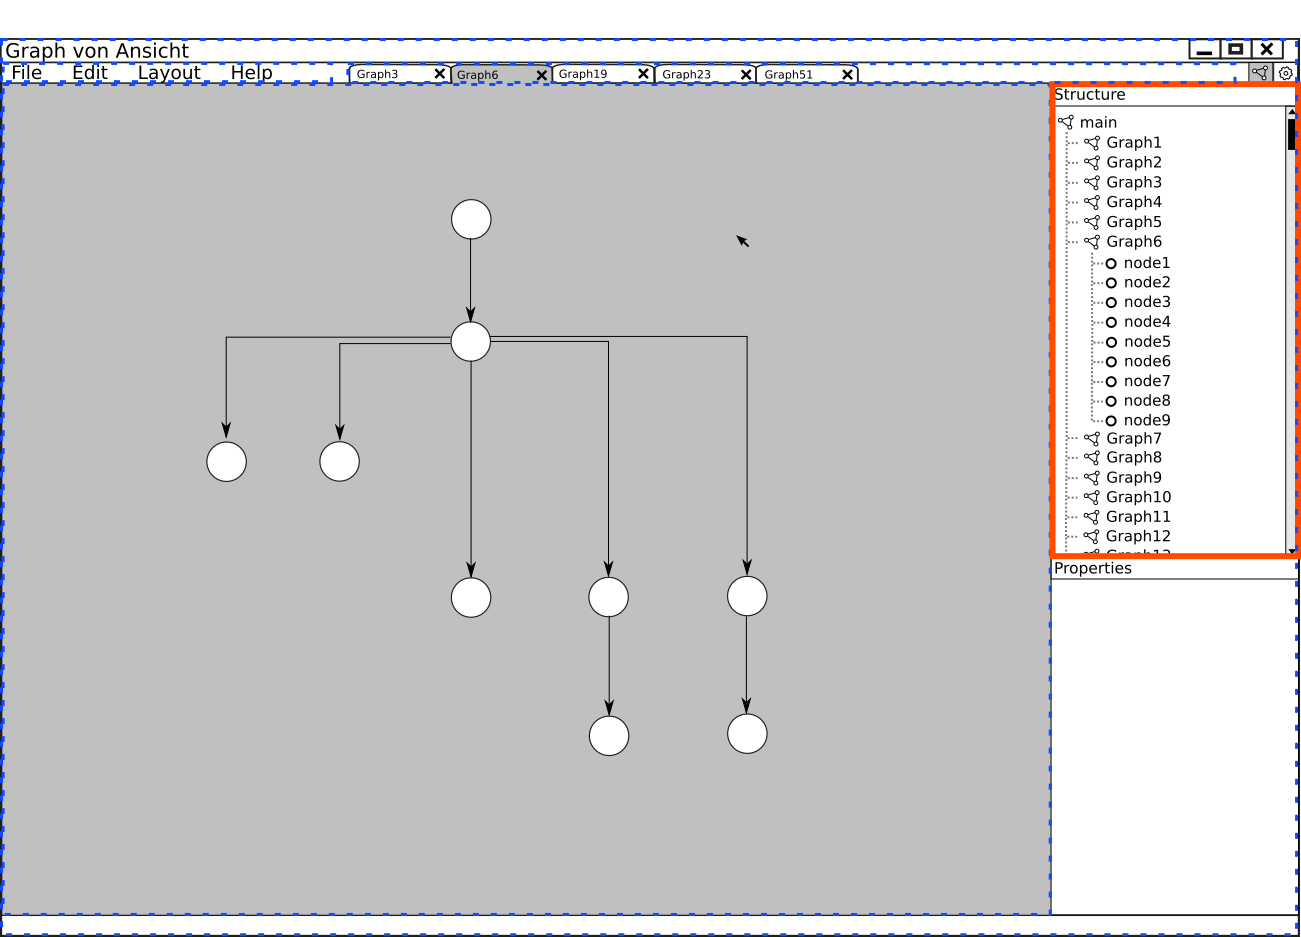
\includegraphics[width=280pt]{resourcen/gui_view_treeview_d.png}}
\end{frame}

\section{Szenario}
\begin{frame}{Szenario}
  \begin{tabular}[t]{cc}
    \begin{minipage}[t]{0.55\textwidth}
      \begin{itemize}
        % Wissenschaftlicher Mitarbeiter möchte den Unterschied eines möglichen Informationslecks im Programmablauf
        % zwischen zwei Änderungen in einem Programm visuell darstellen(Für Paper, Artikel, oder z.B. Lehre)
        \item Importieren der JOANA-Datei %eines Programms das analysiert werden soll
        \pause
        \pause
        \pause
        \item Pfad im Callgraphen verfolgen und/oder Methodengraph öffnen
        \pause
        \pause
        \item Anpassen der Ansicht des Graphen % Einklappen uninteressanter Knoten und Constraint zur übersichtlichen Darstellung der interessanten Knoten hinzufügen
        \pause
        \pause
        \item Exportieren der Ansicht im SVG-Format
        \pause
        \item Informationsleck in der Anwendung schließen % und von JOANA analysieren lassen
        %Einfügen der Grafiken in ein Paper oder wissenschaftlichen Artikel zur Verdeutlichung eines bestimmten Problems und/oder dessen Lösung
      \end{itemize}
  \end{minipage}
    &
    \begin{minipage}[t]{0.35\textwidth}
      \visible<1> {
        \begin{tikzpicture}[remember picture,overlay]
          \node[anchor=east] at (current page.east) {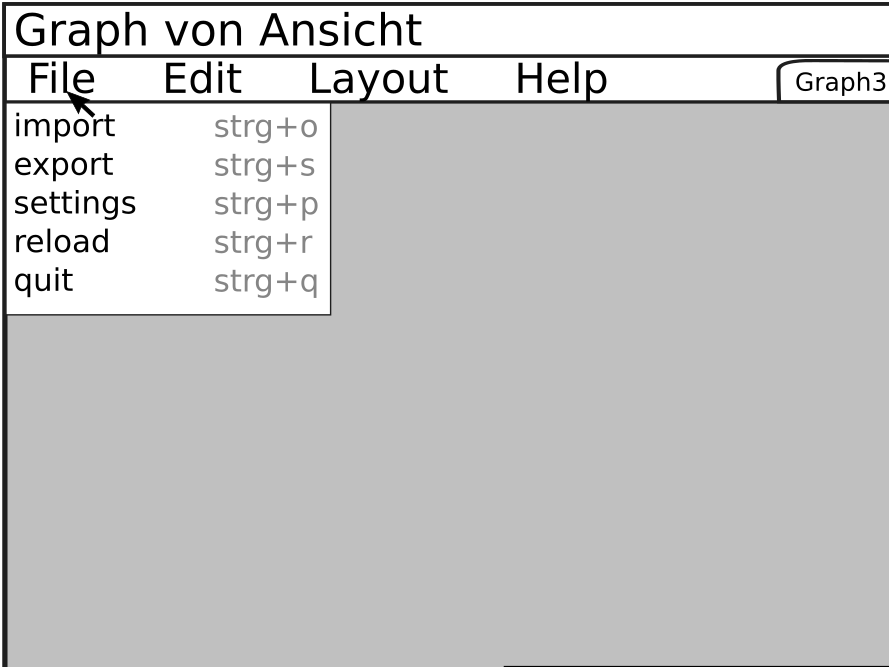
\includegraphics[width=130pt]{resourcen/gui_view_filemenu.png}};
        \end{tikzpicture}
      }
      \visible<2> {
        \begin{tikzpicture}[remember picture,overlay]
          \node[anchor=east] at (current page.east) {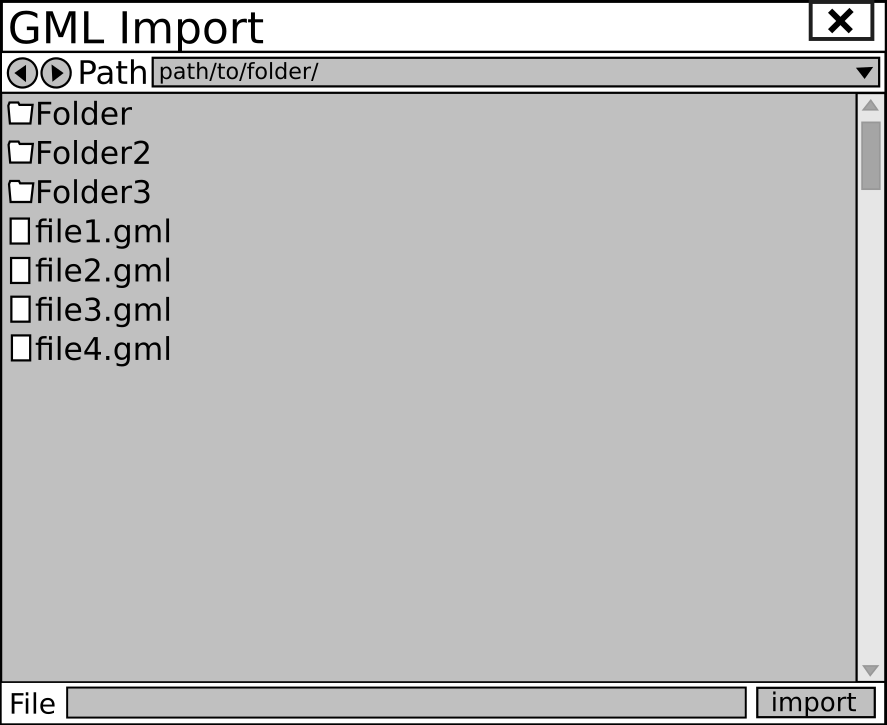
\includegraphics[width=130pt]{resourcen/gui_view_import.png}};
        \end{tikzpicture}
      }
      \visible<3> {
        \begin{tikzpicture}[remember picture,overlay]
          \node[anchor=east] at (current page.east) {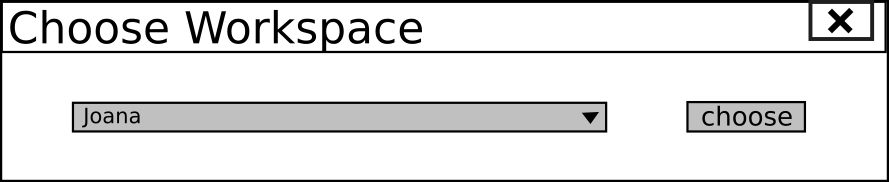
\includegraphics[width=130pt]{resourcen/gui_view_workspace.png}};
        \end{tikzpicture}
      }
      \visible<4> {
        \begin{tikzpicture}[remember picture,overlay]
          \node[anchor=east] at (current page.east) {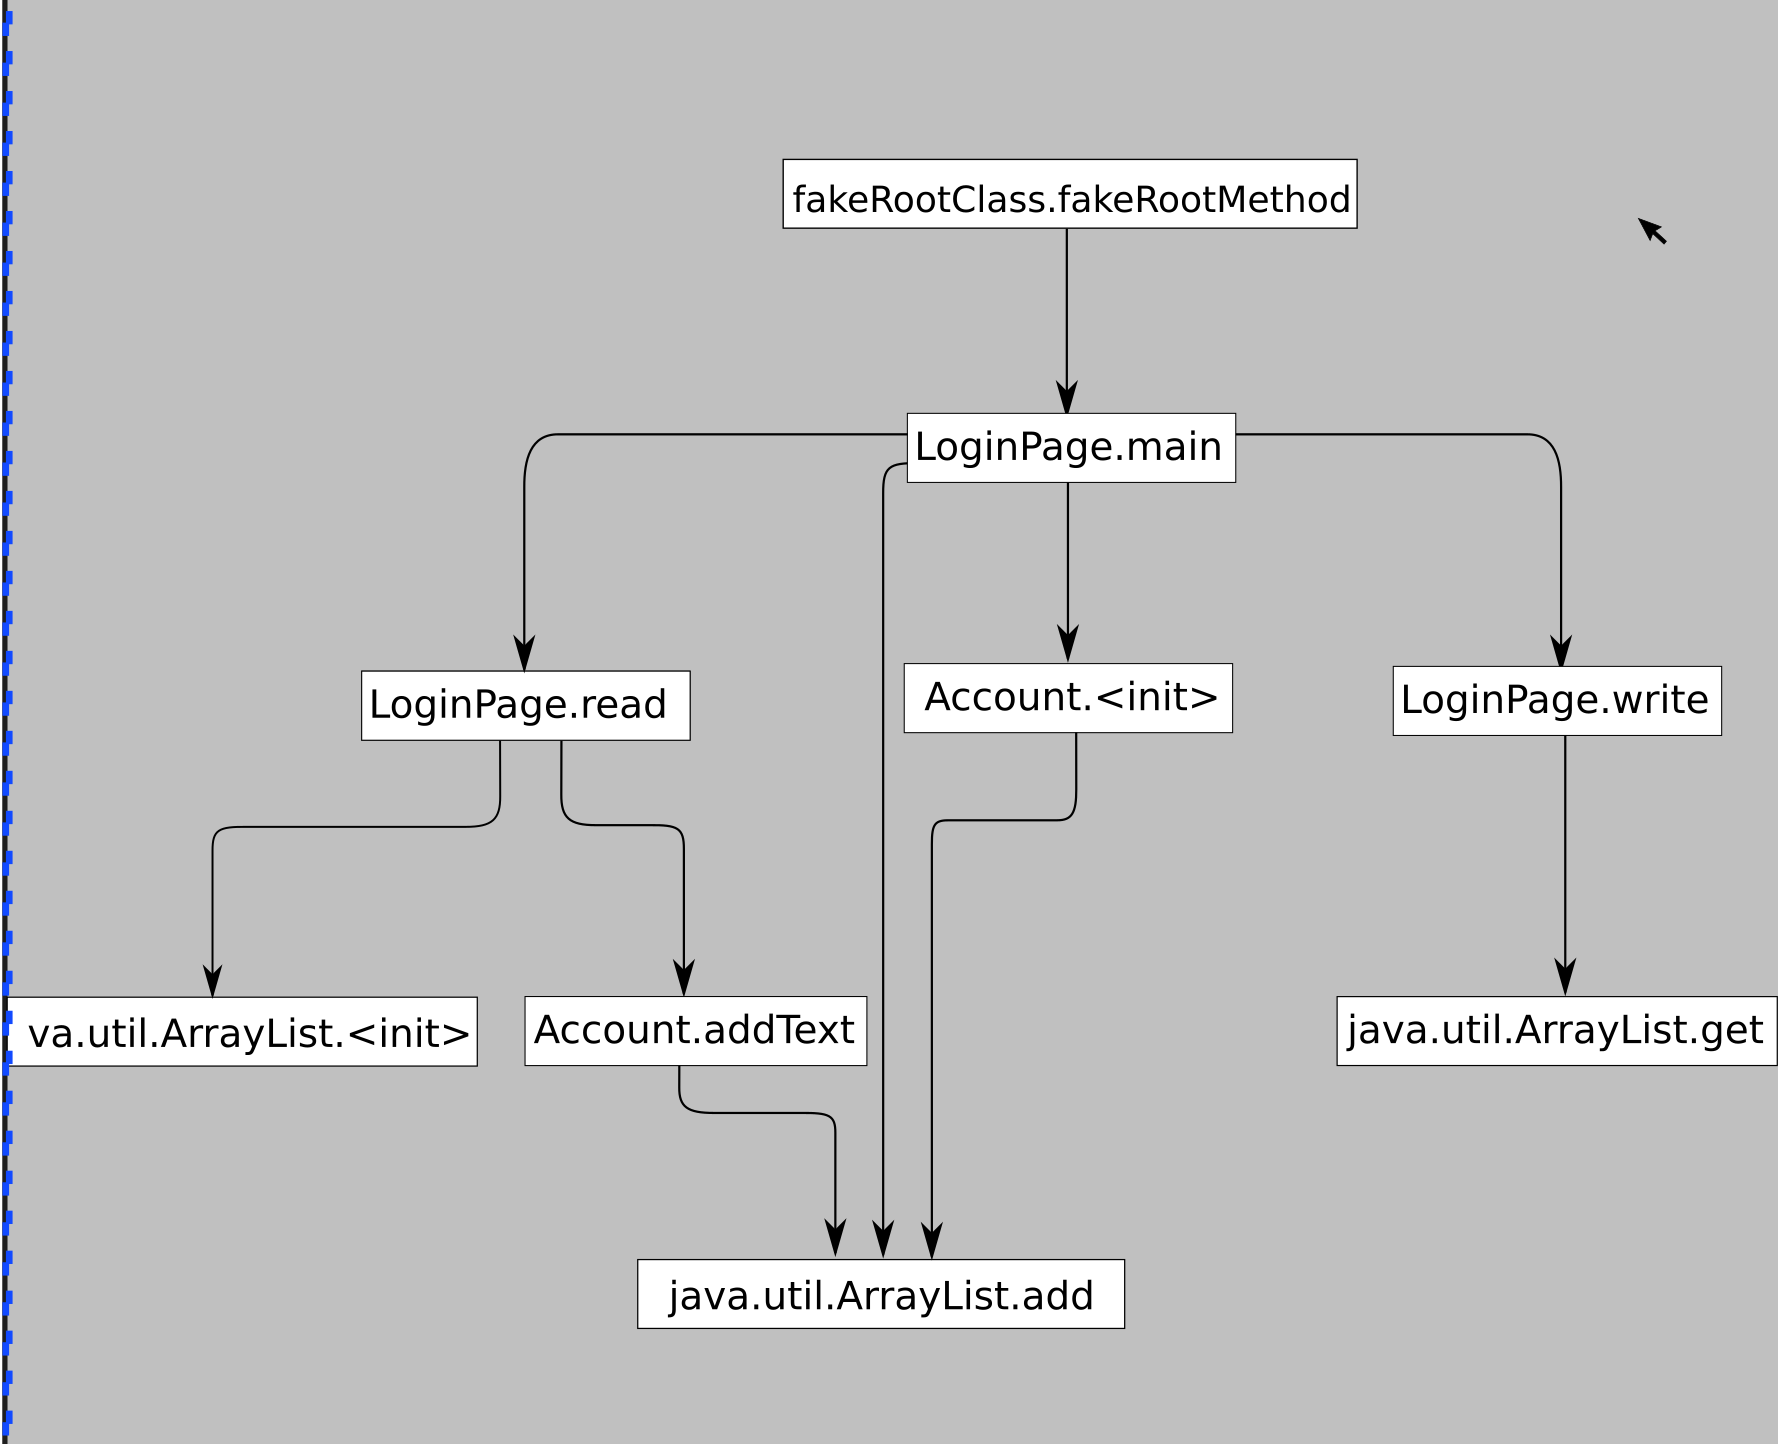
\includegraphics[width=130pt]{resourcen/callgraph.png}};
        \end{tikzpicture}
      }
      \visible<5> {
        \begin{tikzpicture}[remember picture,overlay]
          \node[anchor=east] at (current page.east) {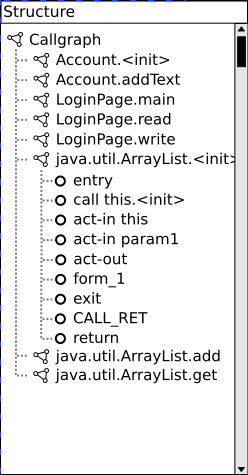
\includegraphics[width=80pt]{resourcen/structureview.png}};
        \end{tikzpicture}
      }
      \visible<6> {
        \begin{tikzpicture}[remember picture,overlay]
          \node[anchor=east] (pfeile) at (current page.east) {
\includegraphics[width=40pt]{resourcen/verschieben.png}};
          \node[anchor=east] at (pfeile.west) {
\includegraphics[width=60pt]{resourcen/lupe.png}};
        \end{tikzpicture}
      }
      \visible<7> {
        \begin{tikzpicture}[remember picture,overlay]
          \node[anchor=east] at (current page.east) {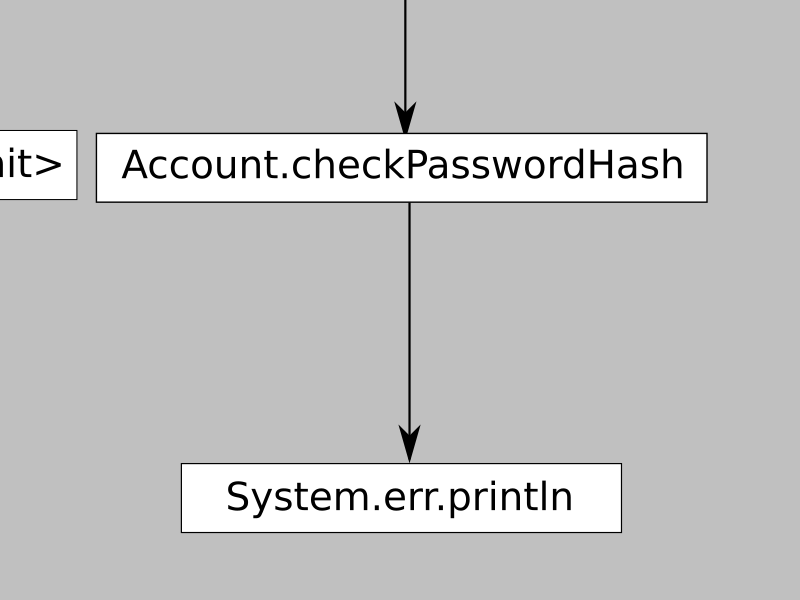
\includegraphics[width=130pt]{resourcen/leak.png}};
        \end{tikzpicture}
      }
      \visible<8> {
        \begin{tikzpicture}[remember picture,overlay]
          \node[anchor=east] at (current page.east) {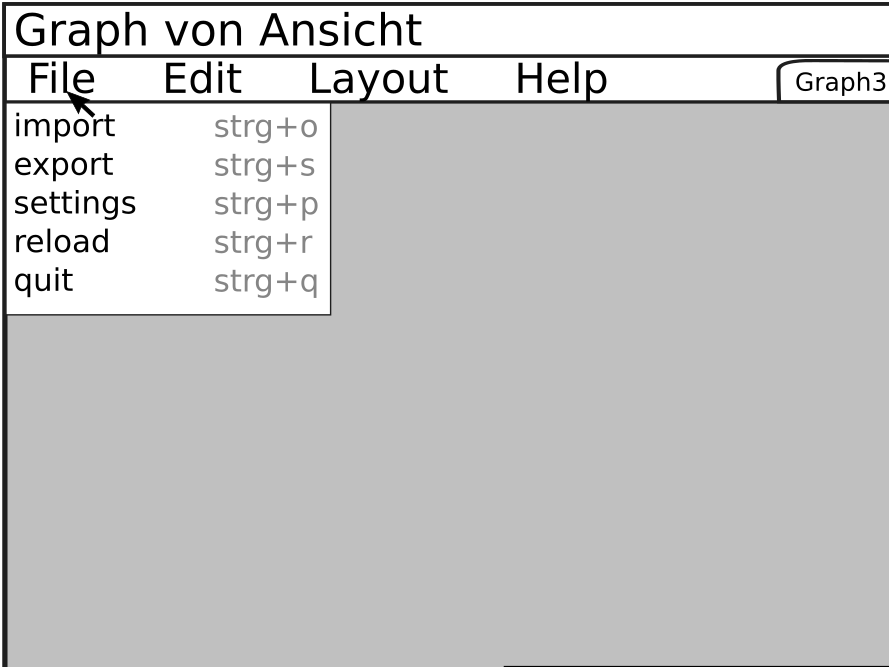
\includegraphics[width=130pt]{resourcen/gui_view_filemenu.png}};
        \end{tikzpicture}
      }
    \end{minipage}
    \\
  \end{tabular}

\end{frame}

\section{Weitere Funktionen}
\begin{frame}{Funktionsübersicht}
  \begin{tabular}[t]{cc}
    \begin{minipage}[t]{0.55\textwidth}
        \begin{itemize}
        \item Parametriesierung des Layouts
        \pause
        \item Ein-/Ausklappen von Subgraphen
        \pause
        \pause
        \item Informationsanzeige zu Knoten, Kanten, Graphen und Subgraphen
        \pause
        \item Mustererkennung von Subgraphen und einheitliche Darstellung
        \pause
        \pause
        \item Filtern bestimmter Knoten- und Kantentypen in der Ansicht
        \pause
      \end{itemize}
  \end{minipage}
    &
    \begin{minipage}[t]{0.35\textwidth}
      \visible<1> {
        \begin{tikzpicture}[remember picture,overlay]
          \node[anchor=east] at (current page.east) {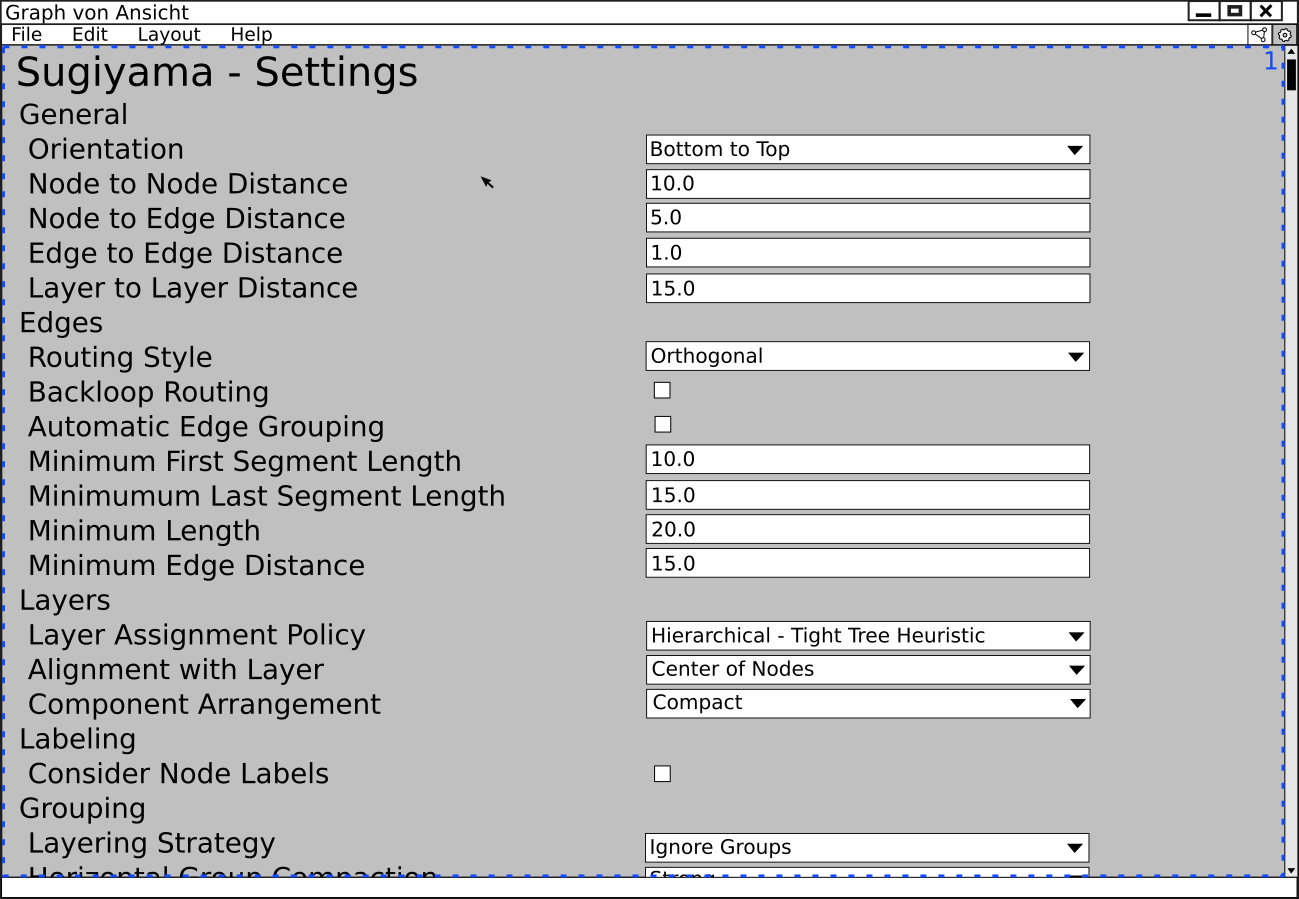
\includegraphics[width=130pt]{gui_layoutsettings_settings.png}};
        \end{tikzpicture}
      }
      \visible<2> {
        \begin{tikzpicture}[remember picture,overlay]
          \node[anchor=east] at (current page.east) {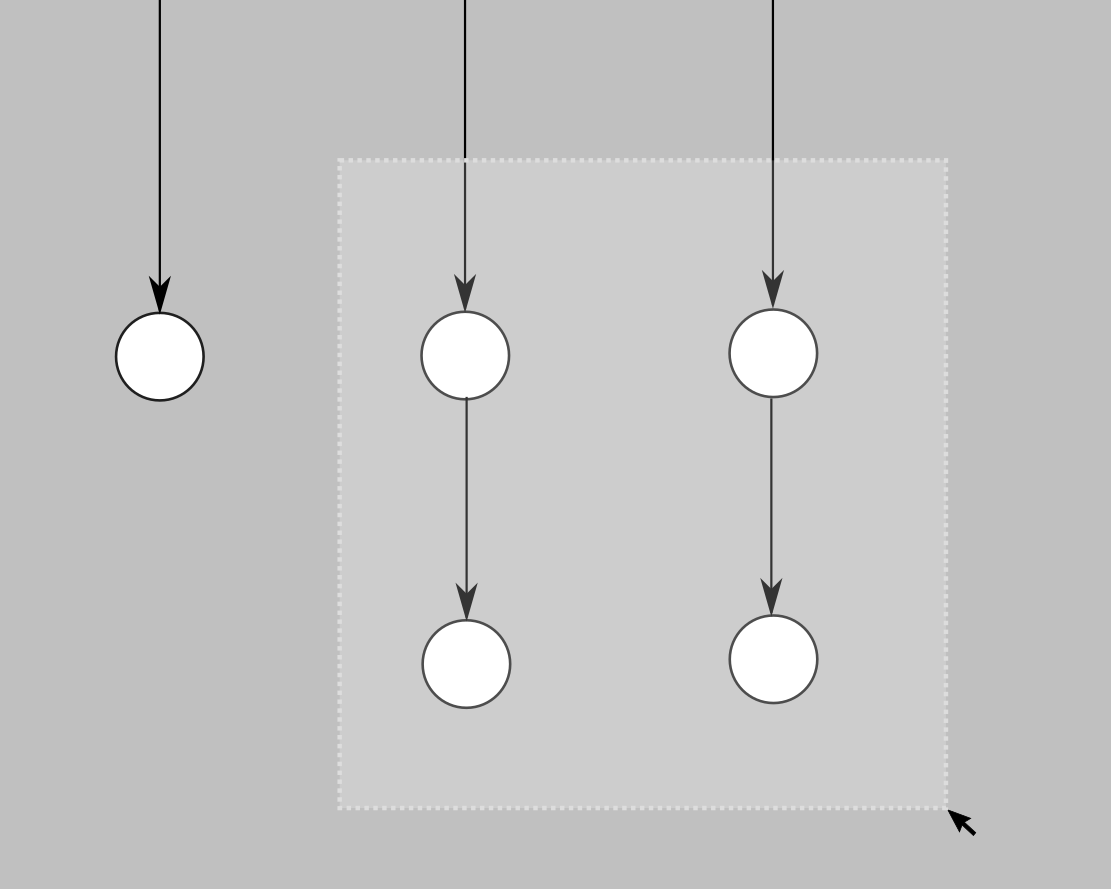
\includegraphics[width=130pt]{resourcen/selection.png}};
        \end{tikzpicture}
      }
      \visible<3> {
        \begin{tikzpicture}[remember picture,overlay]
          \node[anchor=east] at (current page.east) {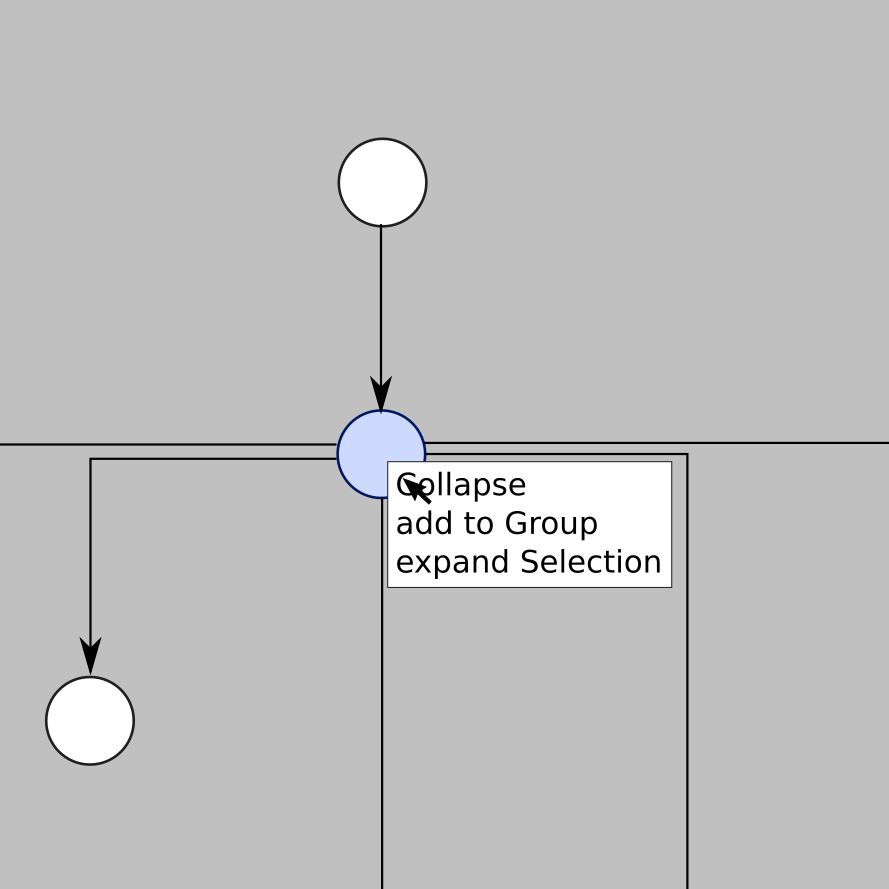
\includegraphics[width=130pt]{resourcen/contextmenu.png}};
        \end{tikzpicture}
      }
      \visible<4> {
        \begin{tikzpicture}[remember picture,overlay]
          \node[anchor=east] at (current page.east) {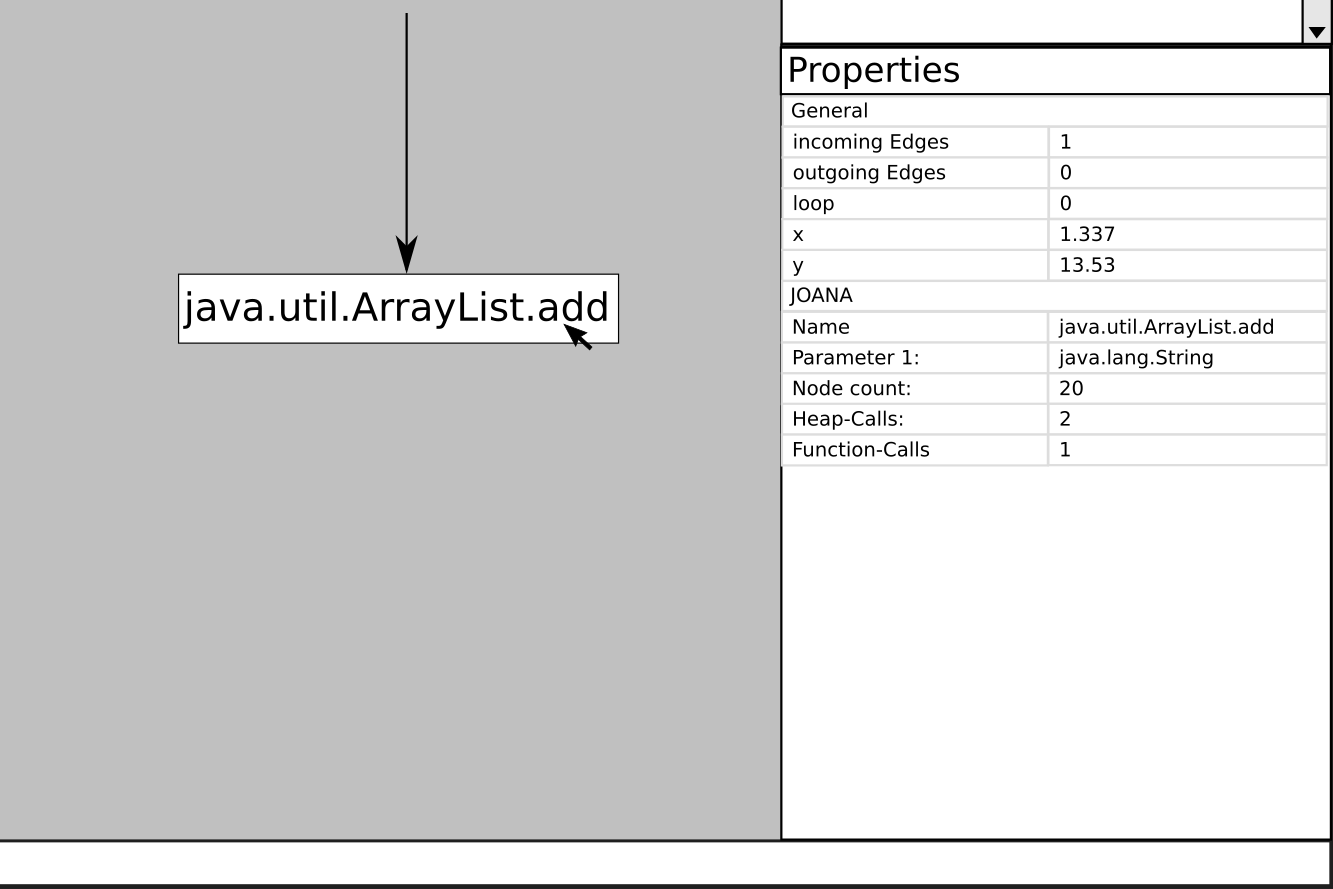
\includegraphics[width=130pt]{resourcen/properties_node.png}};
        \end{tikzpicture}
      }
      \visible<5> {
        \begin{tikzpicture}[remember picture,overlay]
          \node[anchor=east] at (current page.east) {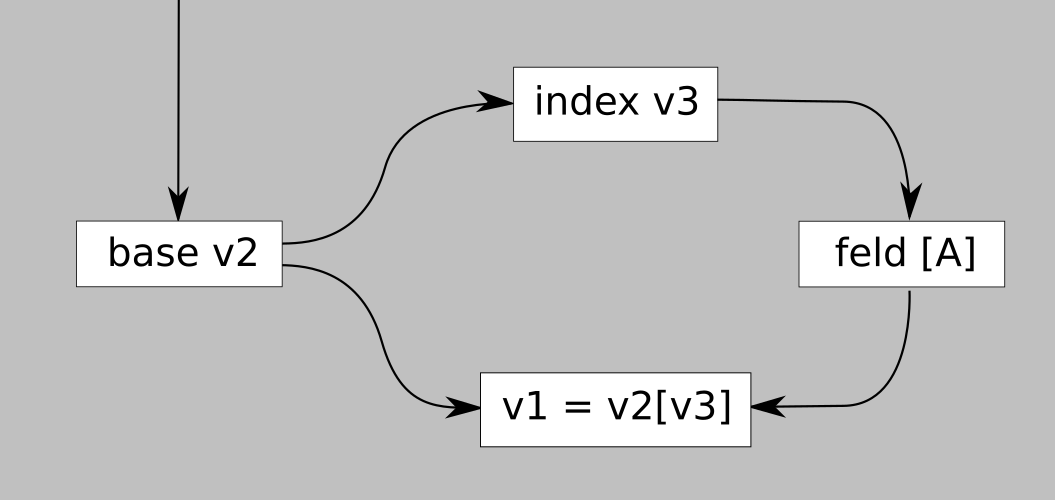
\includegraphics[width=130pt]{resourcen/array_field_access.png}};
        \end{tikzpicture}
      }
      \visible<6> {
        \begin{tikzpicture}[remember picture,overlay]
          \node[anchor=east] at (current page.east) {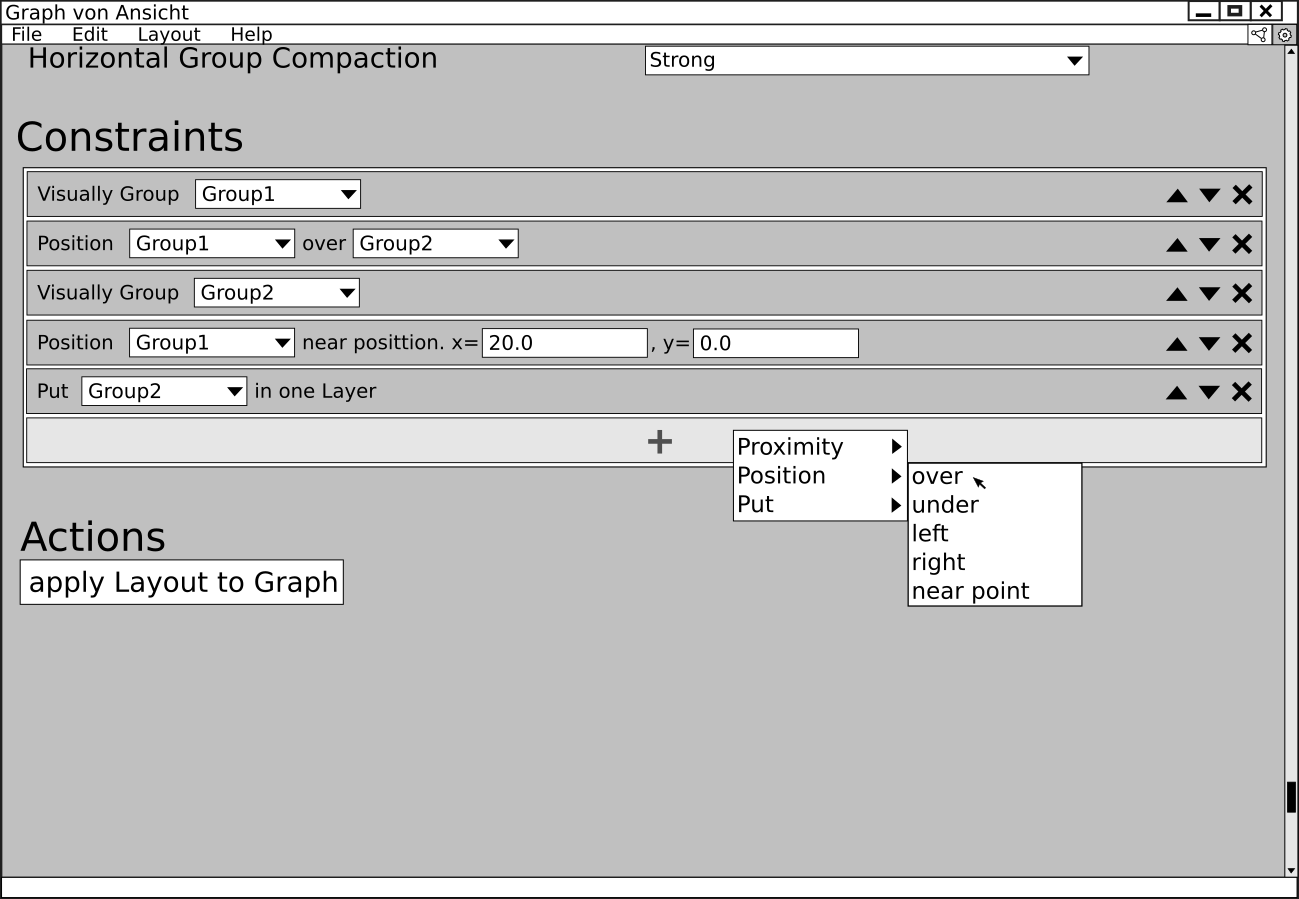
\includegraphics[width=130pt]{gui_layoutsettings_constraints_new.png}};
        \end{tikzpicture}
      }
      \visible<7> {
        \begin{tikzpicture}[remember picture,overlay]
          \node[anchor=east] at (current page.east) {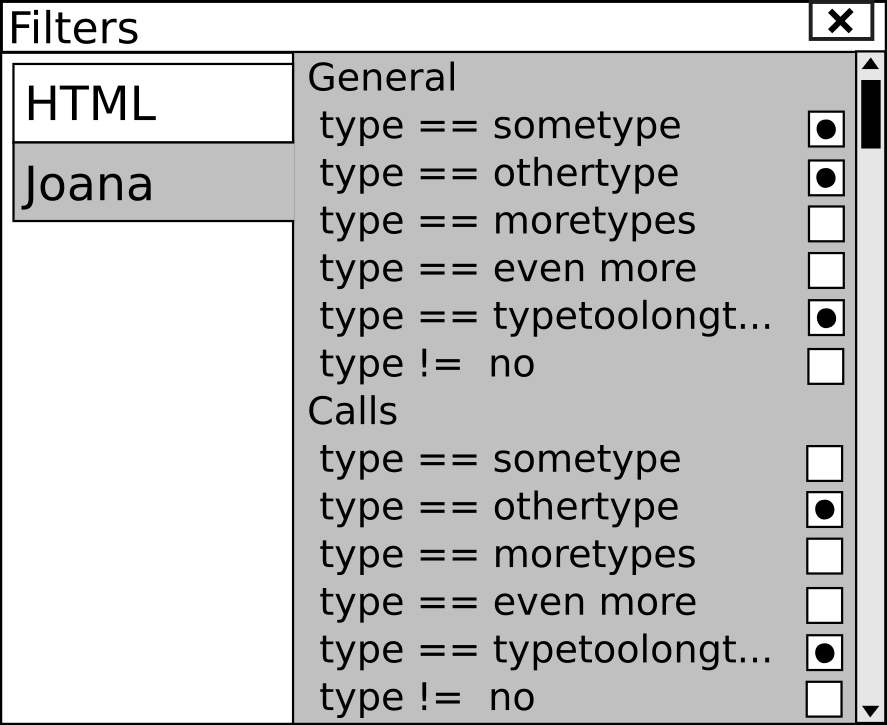
\includegraphics[width=130pt]{resourcen/filters.png}};
        \end{tikzpicture}
      }
    \end{minipage}
    \\
  \end{tabular}

\end{frame}

\appendix

\end{document}
